\documentclass[twoside]{book}

% Packages required by doxygen
\usepackage{fixltx2e}
\usepackage{calc}
\usepackage{doxygen}
\usepackage[export]{adjustbox} % also loads graphicx
\usepackage{graphicx}
\usepackage[utf8]{inputenc}
\usepackage{makeidx}
\usepackage{multicol}
\usepackage{multirow}
\PassOptionsToPackage{warn}{textcomp}
\usepackage{textcomp}
\usepackage[nointegrals]{wasysym}
\usepackage[table]{xcolor}

% Font selection
\usepackage[T1]{fontenc}
\usepackage[scaled=.90]{helvet}
\usepackage{courier}
\usepackage{amssymb}
\usepackage{sectsty}
\renewcommand{\familydefault}{\sfdefault}
\allsectionsfont{%
  \fontseries{bc}\selectfont%
  \color{darkgray}%
}
\renewcommand{\DoxyLabelFont}{%
  \fontseries{bc}\selectfont%
  \color{darkgray}%
}
\newcommand{\+}{\discretionary{\mbox{\scriptsize$\hookleftarrow$}}{}{}}

% Page & text layout
\usepackage{geometry}
\geometry{%
  a4paper,%
  top=2.5cm,%
  bottom=2.5cm,%
  left=2.5cm,%
  right=2.5cm%
}
\tolerance=750
\hfuzz=15pt
\hbadness=750
\setlength{\emergencystretch}{15pt}
\setlength{\parindent}{0cm}
\setlength{\parskip}{3ex plus 2ex minus 2ex}
\makeatletter
\renewcommand{\paragraph}{%
  \@startsection{paragraph}{4}{0ex}{-1.0ex}{1.0ex}{%
    \normalfont\normalsize\bfseries\SS@parafont%
  }%
}
\renewcommand{\subparagraph}{%
  \@startsection{subparagraph}{5}{0ex}{-1.0ex}{1.0ex}{%
    \normalfont\normalsize\bfseries\SS@subparafont%
  }%
}
\makeatother

% Headers & footers
\usepackage{fancyhdr}
\pagestyle{fancyplain}
\fancyhead[LE]{\fancyplain{}{\bfseries\thepage}}
\fancyhead[CE]{\fancyplain{}{}}
\fancyhead[RE]{\fancyplain{}{\bfseries\leftmark}}
\fancyhead[LO]{\fancyplain{}{\bfseries\rightmark}}
\fancyhead[CO]{\fancyplain{}{}}
\fancyhead[RO]{\fancyplain{}{\bfseries\thepage}}
\fancyfoot[LE]{\fancyplain{}{}}
\fancyfoot[CE]{\fancyplain{}{}}
\fancyfoot[RE]{\fancyplain{}{\bfseries\scriptsize Generated by Doxygen }}
\fancyfoot[LO]{\fancyplain{}{\bfseries\scriptsize Generated by Doxygen }}
\fancyfoot[CO]{\fancyplain{}{}}
\fancyfoot[RO]{\fancyplain{}{}}
\renewcommand{\footrulewidth}{0.4pt}
\renewcommand{\chaptermark}[1]{%
  \markboth{#1}{}%
}
\renewcommand{\sectionmark}[1]{%
  \markright{\thesection\ #1}%
}

% Indices & bibliography
\usepackage{natbib}
\usepackage[titles]{tocloft}
\setcounter{tocdepth}{3}
\setcounter{secnumdepth}{5}
\makeindex

% Hyperlinks (required, but should be loaded last)
\usepackage{ifpdf}
\ifpdf
  \usepackage[pdftex,pagebackref=true]{hyperref}
\else
  \usepackage[ps2pdf,pagebackref=true]{hyperref}
\fi
\hypersetup{%
  colorlinks=true,%
  linkcolor=blue,%
  citecolor=blue,%
  unicode%
}

% Custom commands
\newcommand{\clearemptydoublepage}{%
  \newpage{\pagestyle{empty}\cleardoublepage}%
}

\usepackage{caption}
\captionsetup{labelsep=space,justification=centering,font={bf},singlelinecheck=off,skip=4pt,position=top}

%===== C O N T E N T S =====

\begin{document}

% Titlepage & ToC
\hypersetup{pageanchor=false,
             bookmarksnumbered=true,
             pdfencoding=unicode
            }
\pagenumbering{alph}
\begin{titlepage}
\vspace*{7cm}
\begin{center}%
{\Large Indigo }\\
\vspace*{1cm}
{\large Generated by Doxygen 1.8.13}\\
\end{center}
\end{titlepage}
\clearemptydoublepage
\pagenumbering{roman}
\tableofcontents
\clearemptydoublepage
\pagenumbering{arabic}
\hypersetup{pageanchor=true}

%--- Begin generated contents ---
\chapter{Hierarchical Index}
\section{Class Hierarchy}
This inheritance list is sorted roughly, but not completely, alphabetically\+:\begin{DoxyCompactList}
\item \contentsline{section}{Indigo\+:\+:A\+A\+BB}{\pageref{class_indigo_1_1_a_a_b_b}}{}
\item \contentsline{section}{Indigo\+:\+:Application}{\pageref{class_indigo_1_1_application}}{}
\item \contentsline{section}{Indigo\+:\+:Component}{\pageref{class_indigo_1_1_component}}{}
\begin{DoxyCompactList}
\item \contentsline{section}{Indigo\+:\+:Camera}{\pageref{class_indigo_1_1_camera}}{}
\item \contentsline{section}{Indigo\+:\+:Mesh\+Renderer}{\pageref{class_indigo_1_1_mesh_renderer}}{}
\item \contentsline{section}{Indigo\+:\+:Transform}{\pageref{class_indigo_1_1_transform}}{}
\end{DoxyCompactList}
\item \contentsline{section}{Indigo\+:\+:Engine}{\pageref{class_indigo_1_1_engine}}{}
\item \contentsline{section}{Indigo\+:\+:Input}{\pageref{class_indigo_1_1_input}}{}
\item \contentsline{section}{Indigo\+:\+:Mem\+Obj}{\pageref{class_indigo_1_1_mem_obj}}{}
\begin{DoxyCompactList}
\item \contentsline{section}{Indigo\+:\+:Game\+Object}{\pageref{class_indigo_1_1_game_object}}{}
\end{DoxyCompactList}
\item \contentsline{section}{Indigo\+:\+:Mesh}{\pageref{class_indigo_1_1_mesh}}{}
\item \contentsline{section}{Indigo\+:\+:Message}{\pageref{struct_indigo_1_1_message}}{}
\item \contentsline{section}{Indigo\+:\+:Message\+Reg}{\pageref{struct_indigo_1_1_message_reg}}{}
\item \contentsline{section}{plankentry}{\pageref{structplankentry}}{}
\item \contentsline{section}{Indigo\+:\+:Resource}{\pageref{class_indigo_1_1_resource}}{}
\begin{DoxyCompactList}
\item \contentsline{section}{Indigo\+:\+:Mesh\+Resource}{\pageref{class_indigo_1_1_mesh_resource}}{}
\item \contentsline{section}{Indigo\+:\+:Texture\+Resource}{\pageref{class_indigo_1_1_texture_resource}}{}
\end{DoxyCompactList}
\item \contentsline{section}{Indigo\+:\+:Resources}{\pageref{class_indigo_1_1_resources}}{}
\end{DoxyCompactList}

\chapter{Class Index}
\section{Class List}
Here are the classes, structs, unions and interfaces with brief descriptions\+:\begin{DoxyCompactList}
\item\contentsline{section}{\hyperlink{class_indigo_1_1_a_a_b_b}{Indigo\+::\+A\+A\+BB} }{\pageref{class_indigo_1_1_a_a_b_b}}{}
\item\contentsline{section}{\hyperlink{class_indigo_1_1_application}{Indigo\+::\+Application} }{\pageref{class_indigo_1_1_application}}{}
\item\contentsline{section}{\hyperlink{class_indigo_1_1_camera}{Indigo\+::\+Camera} }{\pageref{class_indigo_1_1_camera}}{}
\item\contentsline{section}{\hyperlink{class_indigo_1_1_component}{Indigo\+::\+Component} }{\pageref{class_indigo_1_1_component}}{}
\item\contentsline{section}{\hyperlink{class_indigo_1_1_engine}{Indigo\+::\+Engine} }{\pageref{class_indigo_1_1_engine}}{}
\item\contentsline{section}{\hyperlink{class_indigo_1_1_game_object}{Indigo\+::\+Game\+Object} }{\pageref{class_indigo_1_1_game_object}}{}
\item\contentsline{section}{\hyperlink{class_indigo_1_1_input}{Indigo\+::\+Input} }{\pageref{class_indigo_1_1_input}}{}
\item\contentsline{section}{\hyperlink{class_indigo_1_1_mem_obj}{Indigo\+::\+Mem\+Obj} }{\pageref{class_indigo_1_1_mem_obj}}{}
\item\contentsline{section}{\hyperlink{class_indigo_1_1_mesh}{Indigo\+::\+Mesh} }{\pageref{class_indigo_1_1_mesh}}{}
\item\contentsline{section}{\hyperlink{class_indigo_1_1_mesh_renderer}{Indigo\+::\+Mesh\+Renderer} }{\pageref{class_indigo_1_1_mesh_renderer}}{}
\item\contentsline{section}{\hyperlink{struct_indigo_1_1_message}{Indigo\+::\+Message} }{\pageref{struct_indigo_1_1_message}}{}
\item\contentsline{section}{\hyperlink{struct_indigo_1_1_message_reg}{Indigo\+::\+Message\+Reg} }{\pageref{struct_indigo_1_1_message_reg}}{}
\item\contentsline{section}{\hyperlink{structplankentry}{plankentry} }{\pageref{structplankentry}}{}
\item\contentsline{section}{\hyperlink{class_indigo_1_1_resource}{Indigo\+::\+Resource} }{\pageref{class_indigo_1_1_resource}}{}
\item\contentsline{section}{\hyperlink{class_indigo_1_1_resources}{Indigo\+::\+Resources} }{\pageref{class_indigo_1_1_resources}}{}
\item\contentsline{section}{\hyperlink{class_indigo_1_1_texture}{Indigo\+::\+Texture} }{\pageref{class_indigo_1_1_texture}}{}
\item\contentsline{section}{\hyperlink{class_indigo_1_1_transform}{Indigo\+::\+Transform} }{\pageref{class_indigo_1_1_transform}}{}
\end{DoxyCompactList}

\chapter{Class Documentation}
\hypertarget{class_indigo_1_1_a_a_b_b}{}\section{Indigo\+:\+:A\+A\+BB Class Reference}
\label{class_indigo_1_1_a_a_b_b}\index{Indigo\+::\+A\+A\+BB@{Indigo\+::\+A\+A\+BB}}
\subsection*{Public Member Functions}
\begin{DoxyCompactItemize}
\item 
\mbox{\Hypertarget{class_indigo_1_1_a_a_b_b_abe28ace359bf4c795549f66003277d98}\label{class_indigo_1_1_a_a_b_b_abe28ace359bf4c795549f66003277d98}} 
void {\bfseries Recalc} (std\+::vector$<$ glm\+::vec3 $>$ \+\_\+verts)
\item 
\mbox{\Hypertarget{class_indigo_1_1_a_a_b_b_ad26af46e6323558ba5afd0a1a0ece39c}\label{class_indigo_1_1_a_a_b_b_ad26af46e6323558ba5afd0a1a0ece39c}} 
bool {\bfseries Test} (\hyperlink{class_indigo_1_1_a_a_b_b}{A\+A\+BB} \+\_\+against)
\item 
\mbox{\Hypertarget{class_indigo_1_1_a_a_b_b_a2e2aa4edcee8d263377f29f0bb4b5c48}\label{class_indigo_1_1_a_a_b_b_a2e2aa4edcee8d263377f29f0bb4b5c48}} 
void {\bfseries Set\+Pos} (glm\+::vec3 \+\_\+p)
\item 
\mbox{\Hypertarget{class_indigo_1_1_a_a_b_b_a10b634ba4b56cea6f7e23600f2038399}\label{class_indigo_1_1_a_a_b_b_a10b634ba4b56cea6f7e23600f2038399}} 
void {\bfseries Set\+Scale} (glm\+::vec3 \+\_\+s)
\item 
\mbox{\Hypertarget{class_indigo_1_1_a_a_b_b_a8f012190d6a7dfad085eaf62cb4e084a}\label{class_indigo_1_1_a_a_b_b_a8f012190d6a7dfad085eaf62cb4e084a}} 
void {\bfseries Trans\+Pos} (glm\+::vec3 \+\_\+deltaP)
\end{DoxyCompactItemize}
\subsection*{Static Public Member Functions}
\begin{DoxyCompactItemize}
\item 
\mbox{\Hypertarget{class_indigo_1_1_a_a_b_b_ae37c74a1e633929b06b6cab1fa678451}\label{class_indigo_1_1_a_a_b_b_ae37c74a1e633929b06b6cab1fa678451}} 
static bool {\bfseries Test} (\hyperlink{class_indigo_1_1_a_a_b_b}{A\+A\+BB} \+\_\+a, \hyperlink{class_indigo_1_1_a_a_b_b}{A\+A\+BB} \+\_\+b)
\end{DoxyCompactItemize}


The documentation for this class was generated from the following files\+:\begin{DoxyCompactItemize}
\item 
src/indigo/A\+A\+B\+B.\+h\item 
src/indigo/A\+A\+B\+B.\+cpp\end{DoxyCompactItemize}

\hypertarget{class_indigo_1_1_application}{}\section{Indigo\+:\+:Application Class Reference}
\label{class_indigo_1_1_application}\index{Indigo\+::\+Application@{Indigo\+::\+Application}}
\subsection*{Static Public Member Functions}
\begin{DoxyCompactItemize}
\item 
\mbox{\Hypertarget{class_indigo_1_1_application_a1187d12c4cfd234da50c460eb8f207d7}\label{class_indigo_1_1_application_a1187d12c4cfd234da50c460eb8f207d7}} 
static void {\bfseries Init} (int \+\_\+argc, char $\ast$\+\_\+argv\mbox{[}$\,$\mbox{]})
\item 
\mbox{\Hypertarget{class_indigo_1_1_application_ad9d4706c035d5064ed52eafa9868cf60}\label{class_indigo_1_1_application_ad9d4706c035d5064ed52eafa9868cf60}} 
static void {\bfseries Kill} ()
\item 
\mbox{\Hypertarget{class_indigo_1_1_application_ab64b70bb88997428bb5b49eaa013228f}\label{class_indigo_1_1_application_ab64b70bb88997428bb5b49eaa013228f}} 
static void {\bfseries Shut\+Down} ()
\item 
\mbox{\Hypertarget{class_indigo_1_1_application_aaf09cd6cb412086dc039e28cdb059f0d}\label{class_indigo_1_1_application_aaf09cd6cb412086dc039e28cdb059f0d}} 
static void {\bfseries Run} ()
\item 
\mbox{\Hypertarget{class_indigo_1_1_application_ab0c5855e6fad35691820e44f48eeb319}\label{class_indigo_1_1_application_ab0c5855e6fad35691820e44f48eeb319}} 
static float {\bfseries Get\+DT} ()
\item 
\mbox{\Hypertarget{class_indigo_1_1_application_a7a99ff8c0bd7d815c9596a4ac7a97947}\label{class_indigo_1_1_application_a7a99ff8c0bd7d815c9596a4ac7a97947}} 
static void {\bfseries Err\+Print} (std\+::exception \+\_\+e)
\item 
\mbox{\Hypertarget{class_indigo_1_1_application_a60e0940871b9408b7f8fcc509715e491}\label{class_indigo_1_1_application_a60e0940871b9408b7f8fcc509715e491}} 
static void {\bfseries Err\+Print} (std\+::string \+\_\+msg)
\item 
\mbox{\Hypertarget{class_indigo_1_1_application_a4a09305047e287df89e531fe00e88643}\label{class_indigo_1_1_application_a4a09305047e287df89e531fe00e88643}} 
static void {\bfseries Err\+Print} (G\+Lchar $\ast$\+\_\+msg)
\end{DoxyCompactItemize}
\subsection*{Friends}
\begin{DoxyCompactItemize}
\item 
\mbox{\Hypertarget{class_indigo_1_1_application_a3e1914489e4bed4f9f23cdeab34a43dc}\label{class_indigo_1_1_application_a3e1914489e4bed4f9f23cdeab34a43dc}} 
class {\bfseries Engine}
\item 
\mbox{\Hypertarget{class_indigo_1_1_application_a5b789837fad8c88af8443fc6aa839c75}\label{class_indigo_1_1_application_a5b789837fad8c88af8443fc6aa839c75}} 
class {\bfseries Mem\+Obj}
\item 
\mbox{\Hypertarget{class_indigo_1_1_application_a00df87c957d8f7ee0fc51f07a0542f4a}\label{class_indigo_1_1_application_a00df87c957d8f7ee0fc51f07a0542f4a}} 
class {\bfseries Game\+Object}
\item 
\mbox{\Hypertarget{class_indigo_1_1_application_ad8bd9afbbd7af19d996da80e9d25890d}\label{class_indigo_1_1_application_ad8bd9afbbd7af19d996da80e9d25890d}} 
class {\bfseries Camera}
\end{DoxyCompactItemize}


The documentation for this class was generated from the following files\+:\begin{DoxyCompactItemize}
\item 
src/indigo/Application.\+h\item 
src/indigo/Application.\+cpp\end{DoxyCompactItemize}

\hypertarget{class_indigo_1_1_camera}{}\section{Indigo\+:\+:Camera Class Reference}
\label{class_indigo_1_1_camera}\index{Indigo\+::\+Camera@{Indigo\+::\+Camera}}
Inheritance diagram for Indigo\+:\+:Camera\+:\begin{figure}[H]
\begin{center}
\leavevmode
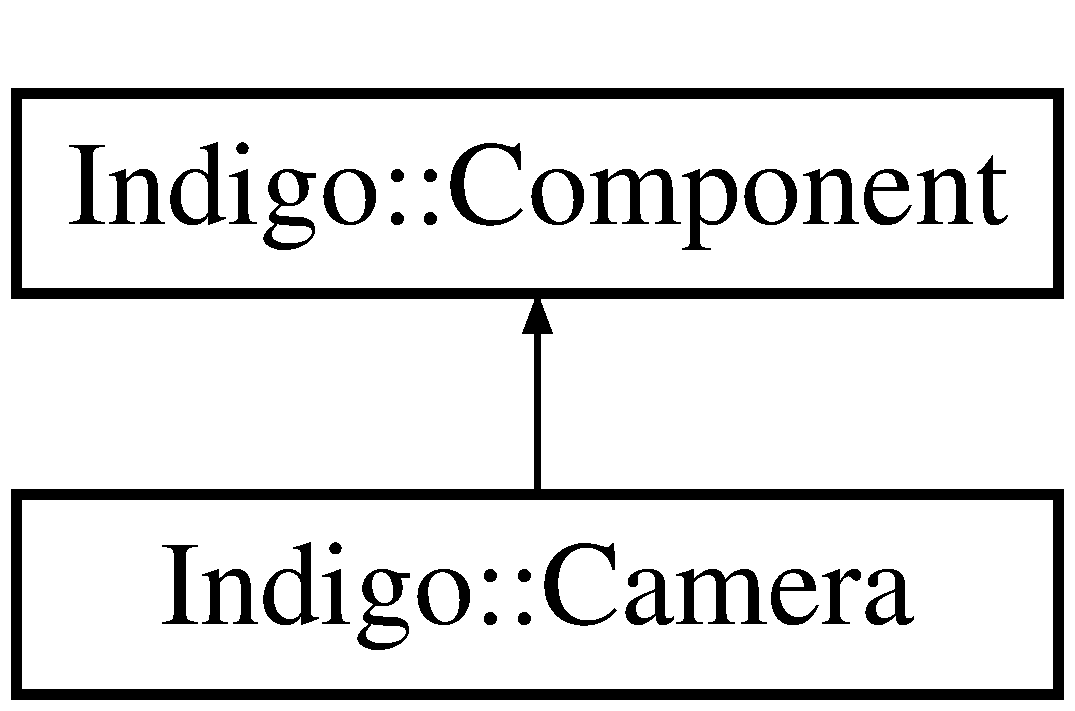
\includegraphics[height=2.000000cm]{class_indigo_1_1_camera}
\end{center}
\end{figure}
\subsection*{Public Member Functions}
\begin{DoxyCompactItemize}
\item 
\mbox{\Hypertarget{class_indigo_1_1_camera_ab99417d5df5a3126910d9b027a9af24b}\label{class_indigo_1_1_camera_ab99417d5df5a3126910d9b027a9af24b}} 
void {\bfseries Render} ()
\end{DoxyCompactItemize}
\subsection*{Friends}
\begin{DoxyCompactItemize}
\item 
\mbox{\Hypertarget{class_indigo_1_1_camera_a3e1914489e4bed4f9f23cdeab34a43dc}\label{class_indigo_1_1_camera_a3e1914489e4bed4f9f23cdeab34a43dc}} 
class {\bfseries Engine}
\end{DoxyCompactItemize}
\subsection*{Additional Inherited Members}


The documentation for this class was generated from the following files\+:\begin{DoxyCompactItemize}
\item 
src/indigo/Camera.\+h\item 
src/indigo/Camera.\+cpp\end{DoxyCompactItemize}

\hypertarget{class_indigo_1_1_component}{}\section{Indigo\+:\+:Component Class Reference}
\label{class_indigo_1_1_component}\index{Indigo\+::\+Component@{Indigo\+::\+Component}}
Inheritance diagram for Indigo\+:\+:Component\+:\begin{figure}[H]
\begin{center}
\leavevmode
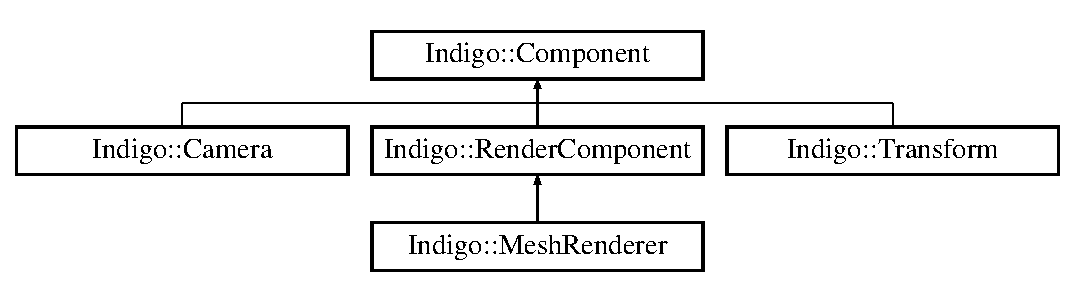
\includegraphics[height=2.000000cm]{class_indigo_1_1_component}
\end{center}
\end{figure}
\subsection*{Public Member Functions}
\begin{DoxyCompactItemize}
\item 
\mbox{\Hypertarget{class_indigo_1_1_component_a4d55fda0bd189f6052934b689ad9c764}\label{class_indigo_1_1_component_a4d55fda0bd189f6052934b689ad9c764}} 
virtual void {\bfseries Update} ()
\item 
\mbox{\Hypertarget{class_indigo_1_1_component_a25c63cb94a289d25074d5b974cef0075}\label{class_indigo_1_1_component_a25c63cb94a289d25074d5b974cef0075}} 
void {\bfseries Parent\+To} (std\+::weak\+\_\+ptr$<$ \hyperlink{class_indigo_1_1_game_object}{Game\+Object} $>$ \+\_\+go)
\end{DoxyCompactItemize}
\subsection*{Protected Attributes}
\begin{DoxyCompactItemize}
\item 
\mbox{\Hypertarget{class_indigo_1_1_component_a2b153d0ff77ec7c38a8881aa4d8cc110}\label{class_indigo_1_1_component_a2b153d0ff77ec7c38a8881aa4d8cc110}} 
std\+::weak\+\_\+ptr$<$ \hyperlink{class_indigo_1_1_game_object}{Game\+Object} $>$ {\bfseries parent}
\end{DoxyCompactItemize}
\subsection*{Friends}
\begin{DoxyCompactItemize}
\item 
\mbox{\Hypertarget{class_indigo_1_1_component_ad8bd9afbbd7af19d996da80e9d25890d}\label{class_indigo_1_1_component_ad8bd9afbbd7af19d996da80e9d25890d}} 
class {\bfseries Camera}
\item 
\mbox{\Hypertarget{class_indigo_1_1_component_a00df87c957d8f7ee0fc51f07a0542f4a}\label{class_indigo_1_1_component_a00df87c957d8f7ee0fc51f07a0542f4a}} 
class {\bfseries Game\+Object}
\end{DoxyCompactItemize}


The documentation for this class was generated from the following files\+:\begin{DoxyCompactItemize}
\item 
src/indigo/Component.\+h\item 
src/indigo/Component.\+cpp\end{DoxyCompactItemize}

\hypertarget{class_indigo_1_1_engine}{}\section{Indigo\+:\+:Engine Class Reference}
\label{class_indigo_1_1_engine}\index{Indigo\+::\+Engine@{Indigo\+::\+Engine}}
\subsection*{Friends}
\begin{DoxyCompactItemize}
\item 
\mbox{\Hypertarget{class_indigo_1_1_engine_a23f25bcc02a0e94c2f5a4188496b04d0}\label{class_indigo_1_1_engine_a23f25bcc02a0e94c2f5a4188496b04d0}} 
class {\bfseries Application}
\item 
\mbox{\Hypertarget{class_indigo_1_1_engine_a5b789837fad8c88af8443fc6aa839c75}\label{class_indigo_1_1_engine_a5b789837fad8c88af8443fc6aa839c75}} 
class {\bfseries Mem\+Obj}
\item 
\mbox{\Hypertarget{class_indigo_1_1_engine_a00df87c957d8f7ee0fc51f07a0542f4a}\label{class_indigo_1_1_engine_a00df87c957d8f7ee0fc51f07a0542f4a}} 
class {\bfseries Game\+Object}
\item 
\mbox{\Hypertarget{class_indigo_1_1_engine_ad8bd9afbbd7af19d996da80e9d25890d}\label{class_indigo_1_1_engine_ad8bd9afbbd7af19d996da80e9d25890d}} 
class {\bfseries Camera}
\end{DoxyCompactItemize}


The documentation for this class was generated from the following files\+:\begin{DoxyCompactItemize}
\item 
src/indigo/Engine.\+h\item 
src/indigo/Engine.\+cpp\end{DoxyCompactItemize}

\hypertarget{class_indigo_1_1_game_object}{}\section{Indigo\+:\+:Game\+Object Class Reference}
\label{class_indigo_1_1_game_object}\index{Indigo\+::\+Game\+Object@{Indigo\+::\+Game\+Object}}
Inheritance diagram for Indigo\+:\+:Game\+Object\+:\begin{figure}[H]
\begin{center}
\leavevmode
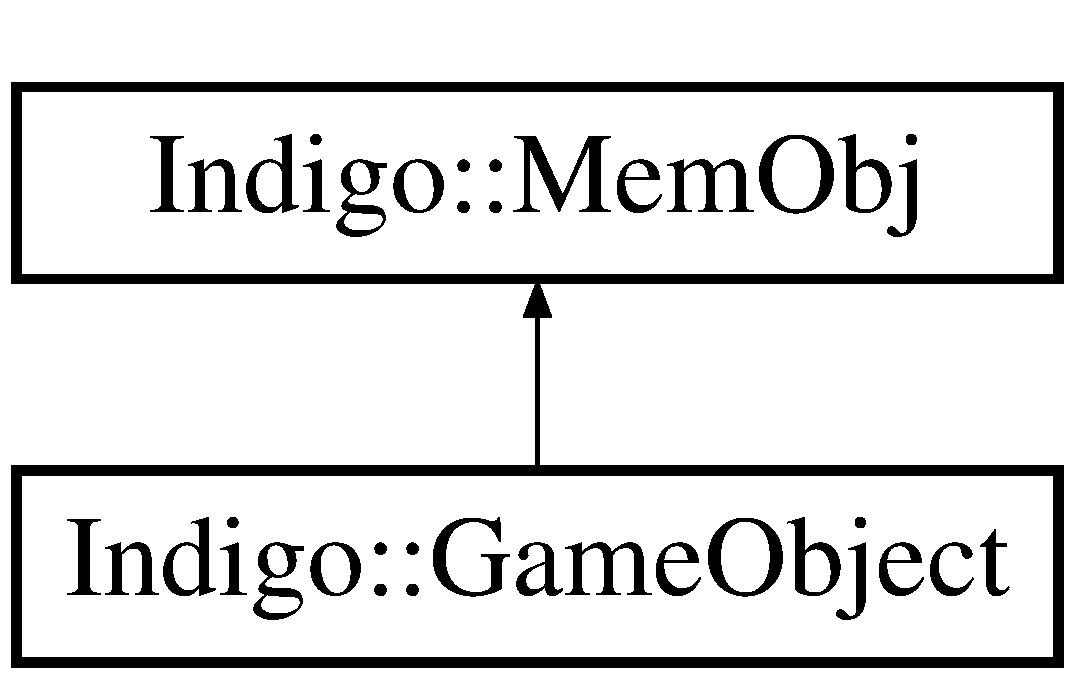
\includegraphics[height=2.000000cm]{class_indigo_1_1_game_object}
\end{center}
\end{figure}
\subsection*{Public Member Functions}
\begin{DoxyCompactItemize}
\item 
\mbox{\Hypertarget{class_indigo_1_1_game_object_a932397dbbf6483a7176ba3e1fce4f44e}\label{class_indigo_1_1_game_object_a932397dbbf6483a7176ba3e1fce4f44e}} 
virtual void {\bfseries on\+Creation} ()
\item 
\mbox{\Hypertarget{class_indigo_1_1_game_object_acd745af3ff2b0e66f812106eb7c4a723}\label{class_indigo_1_1_game_object_acd745af3ff2b0e66f812106eb7c4a723}} 
virtual void {\bfseries on\+Update} ()
\item 
\mbox{\Hypertarget{class_indigo_1_1_game_object_a4cc2ef646c905807df696c5f23ce8d86}\label{class_indigo_1_1_game_object_a4cc2ef646c905807df696c5f23ce8d86}} 
virtual void {\bfseries on\+Late\+Update} ()
\item 
\mbox{\Hypertarget{class_indigo_1_1_game_object_a3c6beac479284b63adf0ee008e5441fa}\label{class_indigo_1_1_game_object_a3c6beac479284b63adf0ee008e5441fa}} 
virtual void {\bfseries Draw} ()
\item 
\mbox{\Hypertarget{class_indigo_1_1_game_object_ae2c7042e5f1617f8ae183415d37c109c}\label{class_indigo_1_1_game_object_ae2c7042e5f1617f8ae183415d37c109c}} 
void {\bfseries Parent\+To} (std\+::weak\+\_\+ptr$<$ \hyperlink{class_indigo_1_1_game_object}{Game\+Object} $>$ \+\_\+go)
\item 
\mbox{\Hypertarget{class_indigo_1_1_game_object_a829a4d75c3ec3ab8d997e004f19ecd75}\label{class_indigo_1_1_game_object_a829a4d75c3ec3ab8d997e004f19ecd75}} 
std\+::weak\+\_\+ptr$<$ \hyperlink{class_indigo_1_1_game_object}{Game\+Object} $>$ {\bfseries Get\+Parent} ()
\item 
\mbox{\Hypertarget{class_indigo_1_1_game_object_ac2716d3d4c2689b075205cd997966557}\label{class_indigo_1_1_game_object_ac2716d3d4c2689b075205cd997966557}} 
{\footnotesize template$<$class T $>$ }\\std\+::weak\+\_\+ptr$<$ T $>$ {\bfseries Add\+Component} ()
\item 
\mbox{\Hypertarget{class_indigo_1_1_game_object_a1cfc6522b37a89a1934a687fa9b4edf2}\label{class_indigo_1_1_game_object_a1cfc6522b37a89a1934a687fa9b4edf2}} 
{\footnotesize template$<$class T $>$ }\\std\+::weak\+\_\+ptr$<$ T $>$ {\bfseries Get\+Component} ()
\item 
\mbox{\Hypertarget{class_indigo_1_1_game_object_a273065f64485474261b8ddffed244bd0}\label{class_indigo_1_1_game_object_a273065f64485474261b8ddffed244bd0}} 
{\footnotesize template$<$class T $>$ }\\std\+::vector$<$ std\+::weak\+\_\+ptr$<$ T $>$ $>$ {\bfseries Get\+Components} ()
\item 
\mbox{\Hypertarget{class_indigo_1_1_game_object_a61c8e0889c22ecf118a7e59daac4002e}\label{class_indigo_1_1_game_object_a61c8e0889c22ecf118a7e59daac4002e}} 
std\+::weak\+\_\+ptr$<$ \hyperlink{class_indigo_1_1_render_component}{Render\+Component} $>$ {\bfseries Get\+Render\+Component} ()
\end{DoxyCompactItemize}
\subsection*{Static Public Member Functions}
\begin{DoxyCompactItemize}
\item 
\mbox{\Hypertarget{class_indigo_1_1_game_object_ac6c3b74cc503f36f7b834f395fd2f2e2}\label{class_indigo_1_1_game_object_ac6c3b74cc503f36f7b834f395fd2f2e2}} 
{\footnotesize template$<$class T $>$ }\\static std\+::weak\+\_\+ptr$<$ T $>$ {\bfseries Create\+Game\+Object} ()
\end{DoxyCompactItemize}
\subsection*{Public Attributes}
\begin{DoxyCompactItemize}
\item 
\mbox{\Hypertarget{class_indigo_1_1_game_object_a807115c579b93b60fbf69a85ac31a65c}\label{class_indigo_1_1_game_object_a807115c579b93b60fbf69a85ac31a65c}} 
std\+::shared\+\_\+ptr$<$ \hyperlink{class_indigo_1_1_transform}{Transform} $>$ {\bfseries transform}
\end{DoxyCompactItemize}
\subsection*{Friends}
\begin{DoxyCompactItemize}
\item 
\mbox{\Hypertarget{class_indigo_1_1_game_object_a3e1914489e4bed4f9f23cdeab34a43dc}\label{class_indigo_1_1_game_object_a3e1914489e4bed4f9f23cdeab34a43dc}} 
class {\bfseries Engine}
\item 
\mbox{\Hypertarget{class_indigo_1_1_game_object_ad8bd9afbbd7af19d996da80e9d25890d}\label{class_indigo_1_1_game_object_ad8bd9afbbd7af19d996da80e9d25890d}} 
class {\bfseries Camera}
\end{DoxyCompactItemize}
\subsection*{Additional Inherited Members}


The documentation for this class was generated from the following files\+:\begin{DoxyCompactItemize}
\item 
src/indigo/Game\+Object.\+h\item 
src/indigo/Game\+Object.\+cpp\end{DoxyCompactItemize}

\hypertarget{class_indigo_1_1_input}{}\section{Indigo\+:\+:Input Class Reference}
\label{class_indigo_1_1_input}\index{Indigo\+::\+Input@{Indigo\+::\+Input}}
\subsection*{Static Public Member Functions}
\begin{DoxyCompactItemize}
\item 
\mbox{\Hypertarget{class_indigo_1_1_input_ac6e91d4097ed5fc3d5a44392f2c1e610}\label{class_indigo_1_1_input_ac6e91d4097ed5fc3d5a44392f2c1e610}} 
static bool {\bfseries Get\+Key} (unsigned char \+\_\+k)
\item 
\mbox{\Hypertarget{class_indigo_1_1_input_ad91170750b641e0e3b371185e9fbd55f}\label{class_indigo_1_1_input_ad91170750b641e0e3b371185e9fbd55f}} 
static bool {\bfseries Get\+Key\+Up} (unsigned char \+\_\+k)
\item 
\mbox{\Hypertarget{class_indigo_1_1_input_a22df61c9b96bbadbd07e255465994a64}\label{class_indigo_1_1_input_a22df61c9b96bbadbd07e255465994a64}} 
static bool {\bfseries Get\+Key\+Down} (unsigned char \+\_\+k)
\end{DoxyCompactItemize}
\subsection*{Friends}
\begin{DoxyCompactItemize}
\item 
\mbox{\Hypertarget{class_indigo_1_1_input_a23f25bcc02a0e94c2f5a4188496b04d0}\label{class_indigo_1_1_input_a23f25bcc02a0e94c2f5a4188496b04d0}} 
class {\bfseries Application}
\end{DoxyCompactItemize}


The documentation for this class was generated from the following files\+:\begin{DoxyCompactItemize}
\item 
src/indigo/Input.\+h\item 
src/indigo/Input.\+cpp\end{DoxyCompactItemize}

\hypertarget{class_indigo_1_1_mem_obj}{}\section{Indigo\+:\+:Mem\+Obj Class Reference}
\label{class_indigo_1_1_mem_obj}\index{Indigo\+::\+Mem\+Obj@{Indigo\+::\+Mem\+Obj}}
Inheritance diagram for Indigo\+:\+:Mem\+Obj\+:\begin{figure}[H]
\begin{center}
\leavevmode
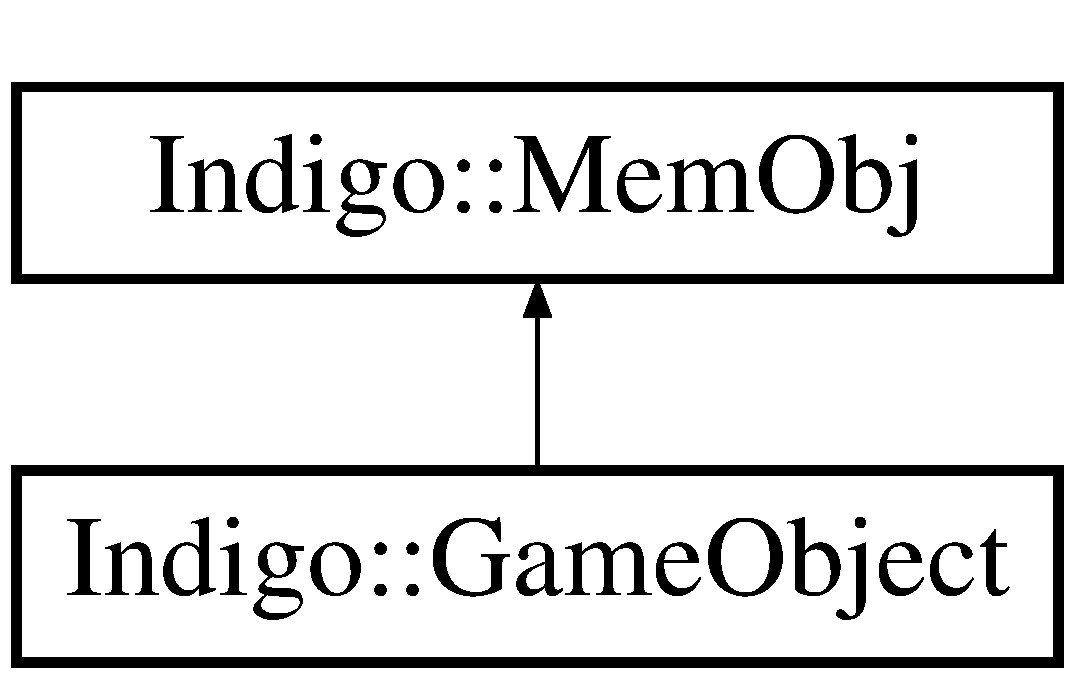
\includegraphics[height=2.000000cm]{class_indigo_1_1_mem_obj}
\end{center}
\end{figure}
\subsection*{Public Member Functions}
\begin{DoxyCompactItemize}
\item 
\mbox{\Hypertarget{class_indigo_1_1_mem_obj_a36b1eb75290fdb4aae51b557660f521d}\label{class_indigo_1_1_mem_obj_a36b1eb75290fdb4aae51b557660f521d}} 
void {\bfseries Mark\+To\+Kill} ()
\item 
\mbox{\Hypertarget{class_indigo_1_1_mem_obj_ad69aa8beafdf695d1e54b6f96dc2b2da}\label{class_indigo_1_1_mem_obj_ad69aa8beafdf695d1e54b6f96dc2b2da}} 
void {\bfseries Send\+Message} (\hyperlink{class_indigo_1_1_mem_obj}{Mem\+Obj} $\ast$\+\_\+to, std\+::string \+\_\+msg)
\item 
\mbox{\Hypertarget{class_indigo_1_1_mem_obj_a71ab9a36e458eb1415016f80c486c48b}\label{class_indigo_1_1_mem_obj_a71ab9a36e458eb1415016f80c486c48b}} 
void {\bfseries Recieve\+Message} (std\+::string \+\_\+msg, std\+::weak\+\_\+ptr$<$ \hyperlink{class_indigo_1_1_mem_obj}{Mem\+Obj} $>$ \+\_\+from)
\end{DoxyCompactItemize}
\subsection*{Protected Member Functions}
\begin{DoxyCompactItemize}
\item 
\mbox{\Hypertarget{class_indigo_1_1_mem_obj_af1d22b7153149088a46a67f1da54b7ab}\label{class_indigo_1_1_mem_obj_af1d22b7153149088a46a67f1da54b7ab}} 
void {\bfseries Register\+Message} (std\+::string \+\_\+msg, void(call)(\hyperlink{class_indigo_1_1_mem_obj}{Mem\+Obj} $\ast$from))
\end{DoxyCompactItemize}
\subsection*{Protected Attributes}
\begin{DoxyCompactItemize}
\item 
\mbox{\Hypertarget{class_indigo_1_1_mem_obj_ace3ed963f343268a689144c4546cac8f}\label{class_indigo_1_1_mem_obj_ace3ed963f343268a689144c4546cac8f}} 
std\+::vector$<$ std\+::string $>$ {\bfseries registered\+Messages}
\end{DoxyCompactItemize}
\subsection*{Friends}
\begin{DoxyCompactItemize}
\item 
\mbox{\Hypertarget{class_indigo_1_1_mem_obj_a3e1914489e4bed4f9f23cdeab34a43dc}\label{class_indigo_1_1_mem_obj_a3e1914489e4bed4f9f23cdeab34a43dc}} 
class {\bfseries Engine}
\end{DoxyCompactItemize}


The documentation for this class was generated from the following files\+:\begin{DoxyCompactItemize}
\item 
src/indigo/Mem\+Obj.\+h\item 
src/indigo/Mem\+Obj.\+cpp\end{DoxyCompactItemize}

\hypertarget{class_indigo_1_1_mesh}{}\section{Indigo\+:\+:Mesh Class Reference}
\label{class_indigo_1_1_mesh}\index{Indigo\+::\+Mesh@{Indigo\+::\+Mesh}}
Inheritance diagram for Indigo\+:\+:Mesh\+:\begin{figure}[H]
\begin{center}
\leavevmode
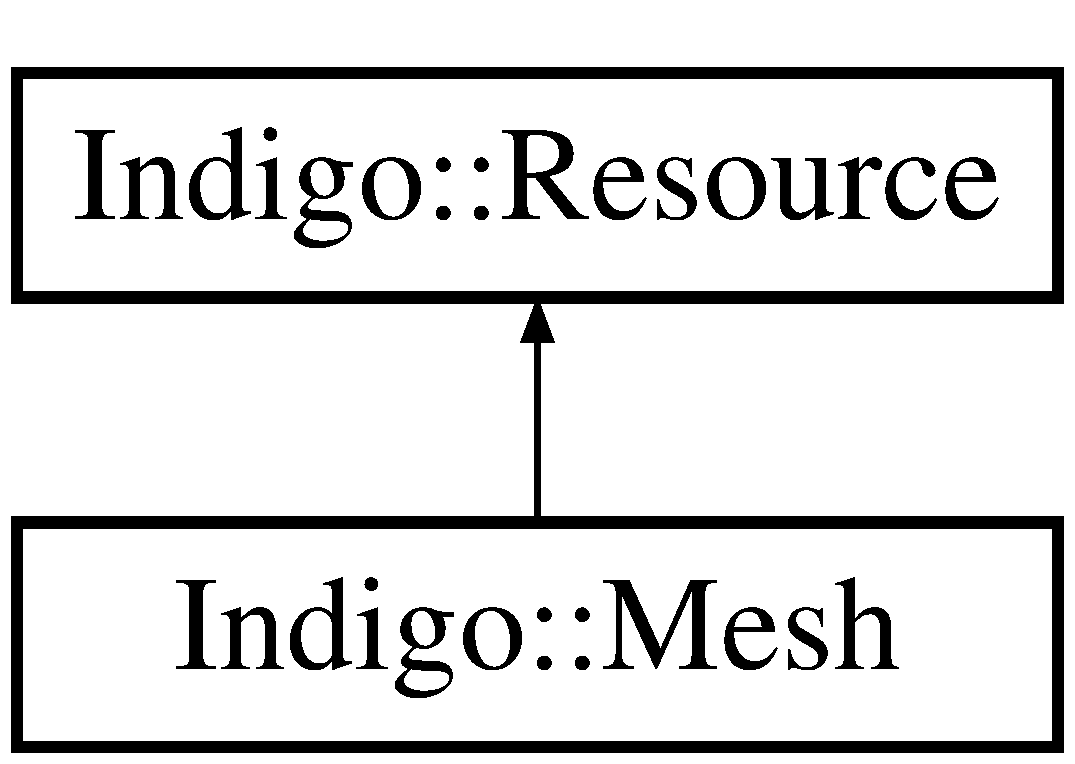
\includegraphics[height=2.000000cm]{class_indigo_1_1_mesh}
\end{center}
\end{figure}
\subsection*{Public Member Functions}
\begin{DoxyCompactItemize}
\item 
\mbox{\Hypertarget{class_indigo_1_1_mesh_a7cd5f7a30e82650d9698a1aa726d2c94}\label{class_indigo_1_1_mesh_a7cd5f7a30e82650d9698a1aa726d2c94}} 
std\+::vector$<$ glm\+::vec3 $>$ $\ast$ {\bfseries Get\+Verts} ()
\end{DoxyCompactItemize}
\subsection*{Friends}
\begin{DoxyCompactItemize}
\item 
\mbox{\Hypertarget{class_indigo_1_1_mesh_a74b3f77e4a7285c624d30192f9643876}\label{class_indigo_1_1_mesh_a74b3f77e4a7285c624d30192f9643876}} 
class {\bfseries Resources}
\end{DoxyCompactItemize}


The documentation for this class was generated from the following file\+:\begin{DoxyCompactItemize}
\item 
src/indigo/Mesh.\+h\end{DoxyCompactItemize}

\hypertarget{class_indigo_1_1_mesh_renderer}{}\section{Indigo\+:\+:Mesh\+Renderer Class Reference}
\label{class_indigo_1_1_mesh_renderer}\index{Indigo\+::\+Mesh\+Renderer@{Indigo\+::\+Mesh\+Renderer}}
Inheritance diagram for Indigo\+:\+:Mesh\+Renderer\+:\begin{figure}[H]
\begin{center}
\leavevmode
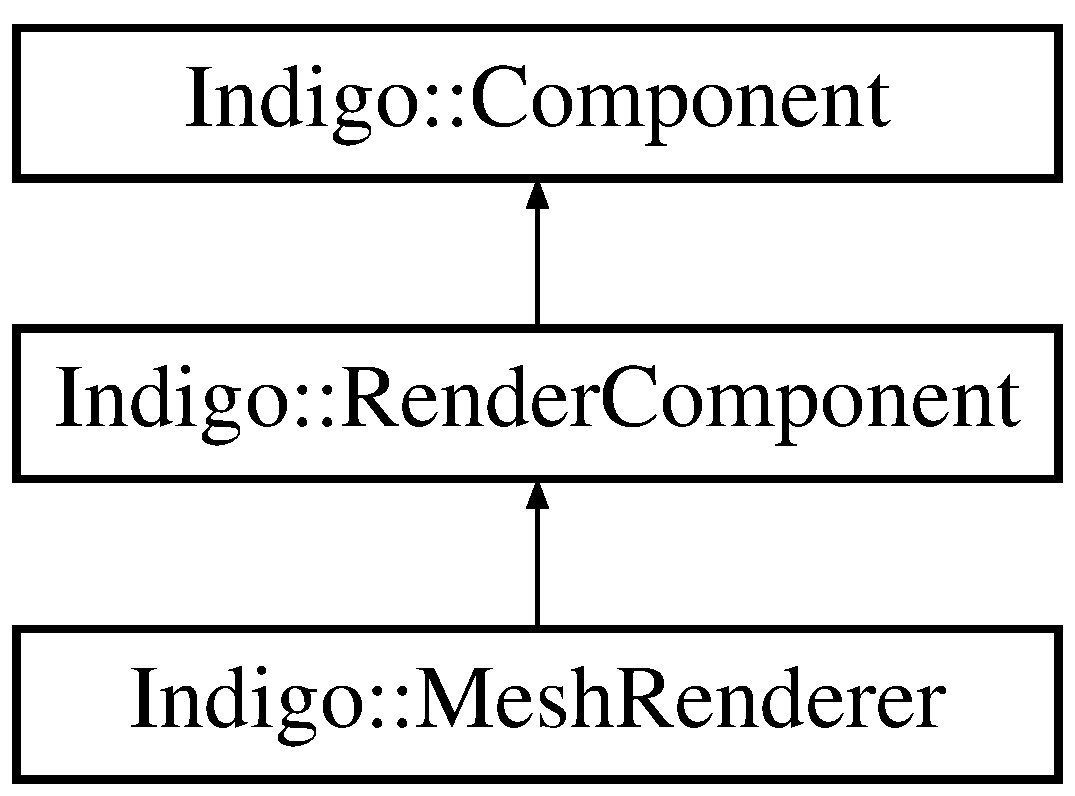
\includegraphics[height=2.000000cm]{class_indigo_1_1_mesh_renderer}
\end{center}
\end{figure}
\subsection*{Public Member Functions}
\begin{DoxyCompactItemize}
\item 
\mbox{\Hypertarget{class_indigo_1_1_mesh_renderer_ae2812e86bacf82ab59875aa2acd8fce9}\label{class_indigo_1_1_mesh_renderer_ae2812e86bacf82ab59875aa2acd8fce9}} 
void {\bfseries Update} ()
\item 
\mbox{\Hypertarget{class_indigo_1_1_mesh_renderer_a42321ee7644cfaeee02b5ba2175b2740}\label{class_indigo_1_1_mesh_renderer_a42321ee7644cfaeee02b5ba2175b2740}} 
void {\bfseries Load\+Mesh} (std\+::string \+\_\+path)
\end{DoxyCompactItemize}
\subsection*{Additional Inherited Members}


The documentation for this class was generated from the following files\+:\begin{DoxyCompactItemize}
\item 
src/indigo/Mesh\+Renderer.\+h\item 
src/indigo/Mesh\+Renderer.\+cpp\end{DoxyCompactItemize}

\hypertarget{class_indigo_1_1_mesh_resource}{}\section{Indigo\+:\+:Mesh\+Resource Class Reference}
\label{class_indigo_1_1_mesh_resource}\index{Indigo\+::\+Mesh\+Resource@{Indigo\+::\+Mesh\+Resource}}
Inheritance diagram for Indigo\+:\+:Mesh\+Resource\+:\begin{figure}[H]
\begin{center}
\leavevmode
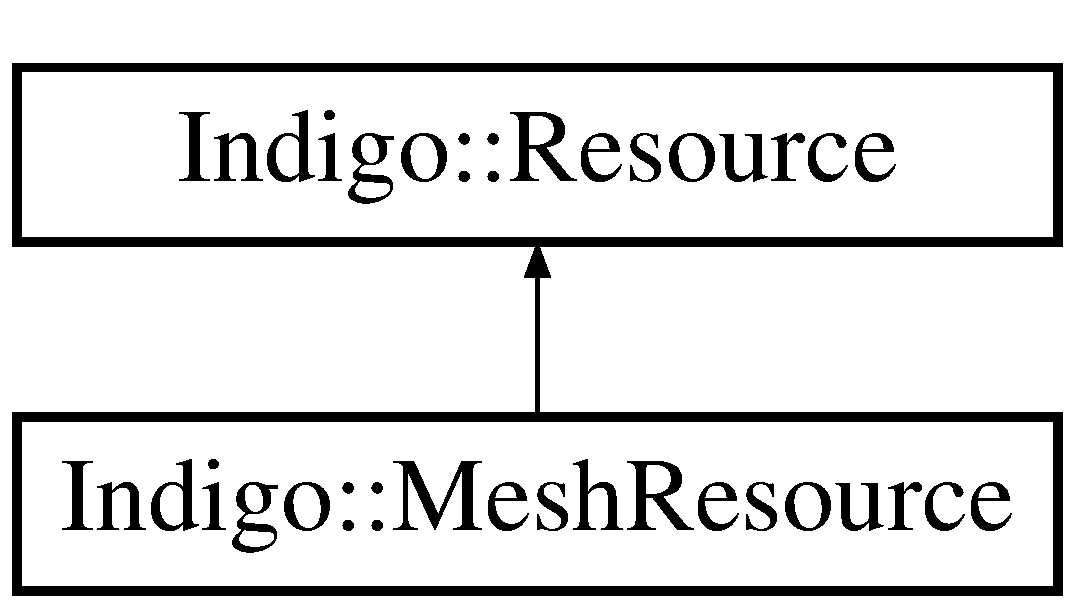
\includegraphics[height=2.000000cm]{class_indigo_1_1_mesh_resource}
\end{center}
\end{figure}
\subsection*{Public Member Functions}
\begin{DoxyCompactItemize}
\item 
\mbox{\Hypertarget{class_indigo_1_1_mesh_resource_a20f924a8ad2ae2618e049ad00a46ea30}\label{class_indigo_1_1_mesh_resource_a20f924a8ad2ae2618e049ad00a46ea30}} 
std\+::vector$<$ glm\+::vec3 $>$ $\ast$ {\bfseries Get\+Verts} ()
\end{DoxyCompactItemize}
\subsection*{Friends}
\begin{DoxyCompactItemize}
\item 
\mbox{\Hypertarget{class_indigo_1_1_mesh_resource_a74b3f77e4a7285c624d30192f9643876}\label{class_indigo_1_1_mesh_resource_a74b3f77e4a7285c624d30192f9643876}} 
class {\bfseries Resources}
\end{DoxyCompactItemize}


The documentation for this class was generated from the following file\+:\begin{DoxyCompactItemize}
\item 
src/indigo/Mesh\+Resource.\+h\end{DoxyCompactItemize}

\hypertarget{class_indigo_1_1_mesh_shader}{}\section{Indigo\+:\+:Mesh\+Shader Class Reference}
\label{class_indigo_1_1_mesh_shader}\index{Indigo\+::\+Mesh\+Shader@{Indigo\+::\+Mesh\+Shader}}
Inheritance diagram for Indigo\+:\+:Mesh\+Shader\+:\begin{figure}[H]
\begin{center}
\leavevmode
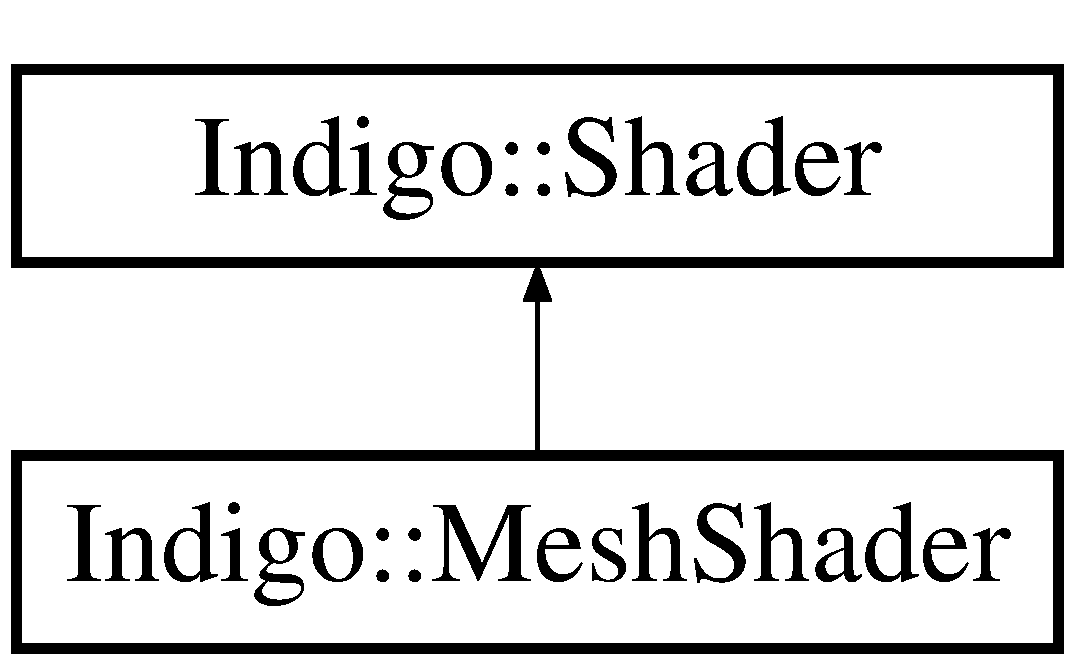
\includegraphics[height=2.000000cm]{class_indigo_1_1_mesh_shader}
\end{center}
\end{figure}
\subsection*{Public Member Functions}
\begin{DoxyCompactItemize}
\item 
\mbox{\Hypertarget{class_indigo_1_1_mesh_shader_af9e4b36e607ce4576432c955dd64a18d}\label{class_indigo_1_1_mesh_shader_af9e4b36e607ce4576432c955dd64a18d}} 
void {\bfseries Load\+Default\+Shaders} ()
\end{DoxyCompactItemize}
\subsection*{Public Attributes}
\begin{DoxyCompactItemize}
\item 
\mbox{\Hypertarget{class_indigo_1_1_mesh_shader_aad885e77e7d755c44426cd3b7a9aca1f}\label{class_indigo_1_1_mesh_shader_aad885e77e7d755c44426cd3b7a9aca1f}} 
G\+Luint {\bfseries mvp\+Handle}
\end{DoxyCompactItemize}
\subsection*{Additional Inherited Members}


The documentation for this class was generated from the following file\+:\begin{DoxyCompactItemize}
\item 
src/indigo/mesh\+Shader.\+h\end{DoxyCompactItemize}

\hypertarget{struct_indigo_1_1_message}{}\section{Indigo\+:\+:Message Struct Reference}
\label{struct_indigo_1_1_message}\index{Indigo\+::\+Message@{Indigo\+::\+Message}}
\subsection*{Public Attributes}
\begin{DoxyCompactItemize}
\item 
\mbox{\Hypertarget{struct_indigo_1_1_message_a8c6243e6147e6adb9e550dab5544746d}\label{struct_indigo_1_1_message_a8c6243e6147e6adb9e550dab5544746d}} 
std\+::weak\+\_\+ptr$<$ \hyperlink{class_indigo_1_1_mem_obj}{Mem\+Obj} $>$ {\bfseries from}
\item 
\mbox{\Hypertarget{struct_indigo_1_1_message_aefdd64f0fa7ce7f8fa955ce9242b82de}\label{struct_indigo_1_1_message_aefdd64f0fa7ce7f8fa955ce9242b82de}} 
std\+::weak\+\_\+ptr$<$ \hyperlink{class_indigo_1_1_mem_obj}{Mem\+Obj} $>$ {\bfseries to}
\item 
\mbox{\Hypertarget{struct_indigo_1_1_message_aca5d32719ecc9366f536d9947273f36e}\label{struct_indigo_1_1_message_aca5d32719ecc9366f536d9947273f36e}} 
std\+::string {\bfseries msg}
\end{DoxyCompactItemize}


The documentation for this struct was generated from the following file\+:\begin{DoxyCompactItemize}
\item 
src/indigo/message.\+h\end{DoxyCompactItemize}

\hypertarget{struct_indigo_1_1_message_reg}{}\section{Indigo\+:\+:Message\+Reg Struct Reference}
\label{struct_indigo_1_1_message_reg}\index{Indigo\+::\+Message\+Reg@{Indigo\+::\+Message\+Reg}}
\subsection*{Public Attributes}
\begin{DoxyCompactItemize}
\item 
\mbox{\Hypertarget{struct_indigo_1_1_message_reg_ae861511f1aaae96c3c4846cfa21e2643}\label{struct_indigo_1_1_message_reg_ae861511f1aaae96c3c4846cfa21e2643}} 
std\+::string {\bfseries msg}
\item 
\mbox{\Hypertarget{struct_indigo_1_1_message_reg_a9da66eba103cd9085803686d5f180906}\label{struct_indigo_1_1_message_reg_a9da66eba103cd9085803686d5f180906}} 
void($\ast$ {\bfseries callback} )(\hyperlink{class_indigo_1_1_mem_obj}{Mem\+Obj} $\ast$from)
\end{DoxyCompactItemize}


The documentation for this struct was generated from the following file\+:\begin{DoxyCompactItemize}
\item 
src/indigo/Mem\+Obj.\+h\end{DoxyCompactItemize}

\hypertarget{structplankentry}{}\section{plankentry Struct Reference}
\label{structplankentry}\index{plankentry@{plankentry}}
\subsection*{Public Attributes}
\begin{DoxyCompactItemize}
\item 
\mbox{\Hypertarget{structplankentry_a16d8d18966483144fc49e496e75cdfa6}\label{structplankentry_a16d8d18966483144fc49e496e75cdfa6}} 
void $\ast$ {\bfseries ptr}
\item 
\mbox{\Hypertarget{structplankentry_a22ad83e491df0cc6e747c4388166cdcb}\label{structplankentry_a22ad83e491df0cc6e747c4388166cdcb}} 
size\+\_\+t {\bfseries size}
\item 
\mbox{\Hypertarget{structplankentry_a296c7c00bbd98a52896d8f1c7d5b3d20}\label{structplankentry_a296c7c00bbd98a52896d8f1c7d5b3d20}} 
\hyperlink{structplankentry}{plankentry} $\ast$ {\bfseries next}
\end{DoxyCompactItemize}


The documentation for this struct was generated from the following file\+:\begin{DoxyCompactItemize}
\item 
src/indigo/plank.\+cpp\end{DoxyCompactItemize}

\hypertarget{class_indigo_1_1_render_component}{}\section{Indigo\+:\+:Render\+Component Class Reference}
\label{class_indigo_1_1_render_component}\index{Indigo\+::\+Render\+Component@{Indigo\+::\+Render\+Component}}
Inheritance diagram for Indigo\+:\+:Render\+Component\+:\begin{figure}[H]
\begin{center}
\leavevmode
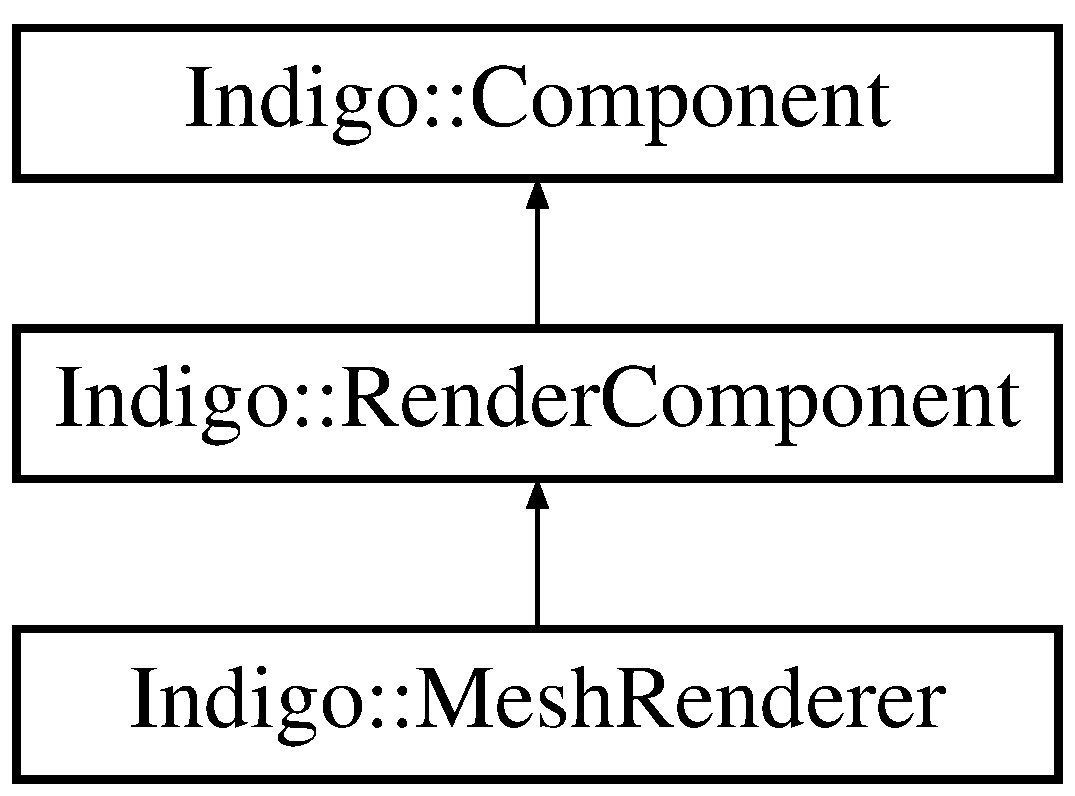
\includegraphics[height=3.000000cm]{class_indigo_1_1_render_component}
\end{center}
\end{figure}
\subsection*{Public Member Functions}
\begin{DoxyCompactItemize}
\item 
\mbox{\Hypertarget{class_indigo_1_1_render_component_af2e372cfda77bb739b44f1ae81a8009b}\label{class_indigo_1_1_render_component_af2e372cfda77bb739b44f1ae81a8009b}} 
virtual void {\bfseries Draw} ()
\end{DoxyCompactItemize}
\subsection*{Additional Inherited Members}


The documentation for this class was generated from the following file\+:\begin{DoxyCompactItemize}
\item 
src/indigo/Render\+Component.\+h\end{DoxyCompactItemize}

\hypertarget{class_indigo_1_1_resource}{}\section{Indigo\+:\+:Resource Class Reference}
\label{class_indigo_1_1_resource}\index{Indigo\+::\+Resource@{Indigo\+::\+Resource}}
Inheritance diagram for Indigo\+:\+:Resource\+:\begin{figure}[H]
\begin{center}
\leavevmode
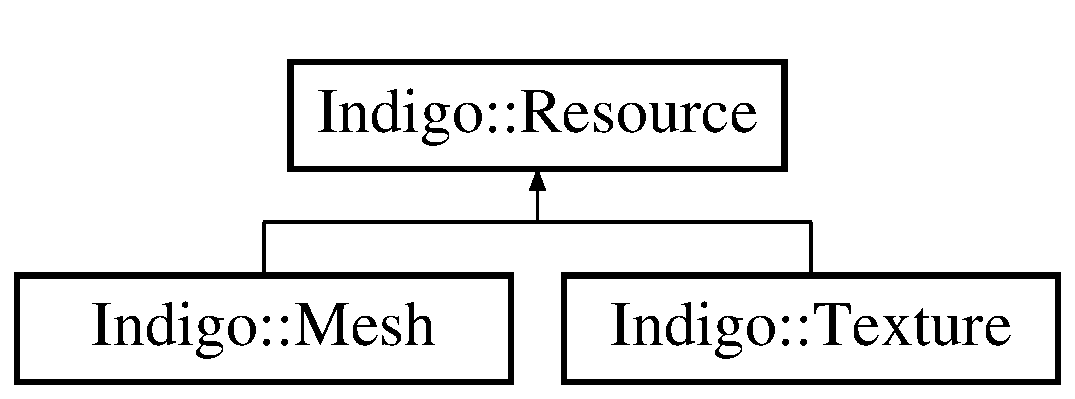
\includegraphics[height=2.000000cm]{class_indigo_1_1_resource}
\end{center}
\end{figure}
\subsection*{Friends}
\begin{DoxyCompactItemize}
\item 
\mbox{\Hypertarget{class_indigo_1_1_resource_a74b3f77e4a7285c624d30192f9643876}\label{class_indigo_1_1_resource_a74b3f77e4a7285c624d30192f9643876}} 
class {\bfseries Resources}
\end{DoxyCompactItemize}


The documentation for this class was generated from the following file\+:\begin{DoxyCompactItemize}
\item 
src/indigo/resource.\+h\end{DoxyCompactItemize}

\hypertarget{class_indigo_1_1_resources}{}\section{Indigo\+:\+:Resources Class Reference}
\label{class_indigo_1_1_resources}\index{Indigo\+::\+Resources@{Indigo\+::\+Resources}}
\subsection*{Static Public Member Functions}
\begin{DoxyCompactItemize}
\item 
\mbox{\Hypertarget{class_indigo_1_1_resources_a22b34571bcf56685cff314cf20f333a8}\label{class_indigo_1_1_resources_a22b34571bcf56685cff314cf20f333a8}} 
static std\+::weak\+\_\+ptr$<$ \hyperlink{class_indigo_1_1_mesh_resource}{Mesh\+Resource} $>$ {\bfseries Load\+Mesh} (std\+::string \+\_\+path)
\item 
\mbox{\Hypertarget{class_indigo_1_1_resources_a53c3ca210d85b35b97d9179c641a7261}\label{class_indigo_1_1_resources_a53c3ca210d85b35b97d9179c641a7261}} 
static std\+::weak\+\_\+ptr$<$ \hyperlink{class_indigo_1_1_texture_resource}{Texture\+Resource} $>$ {\bfseries Load\+Texture} (std\+::string \+\_\+path)
\end{DoxyCompactItemize}


The documentation for this class was generated from the following files\+:\begin{DoxyCompactItemize}
\item 
src/indigo/Resources.\+h\item 
src/indigo/Resources.\+cpp\end{DoxyCompactItemize}

\hypertarget{class_indigo_1_1_shader}{}\section{Indigo\+:\+:Shader Class Reference}
\label{class_indigo_1_1_shader}\index{Indigo\+::\+Shader@{Indigo\+::\+Shader}}
Inheritance diagram for Indigo\+:\+:Shader\+:\begin{figure}[H]
\begin{center}
\leavevmode
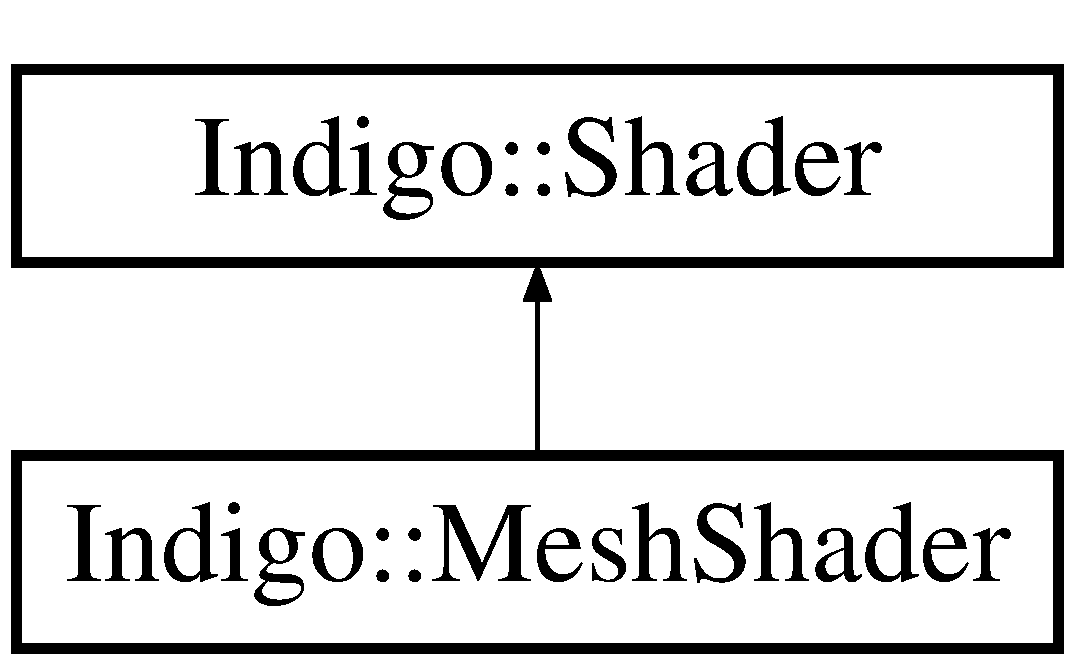
\includegraphics[height=2.000000cm]{class_indigo_1_1_shader}
\end{center}
\end{figure}
\subsection*{Public Member Functions}
\begin{DoxyCompactItemize}
\item 
\mbox{\Hypertarget{class_indigo_1_1_shader_a9143ecbc145cc7d16f0ccd352e576540}\label{class_indigo_1_1_shader_a9143ecbc145cc7d16f0ccd352e576540}} 
void {\bfseries Init} ()
\item 
\mbox{\Hypertarget{class_indigo_1_1_shader_a4315a6336472b293392aa50e7a4e65d0}\label{class_indigo_1_1_shader_a4315a6336472b293392aa50e7a4e65d0}} 
void {\bfseries Activate} ()
\item 
\mbox{\Hypertarget{class_indigo_1_1_shader_a49b6c5b41ca89e0888b5e72903a5a02e}\label{class_indigo_1_1_shader_a49b6c5b41ca89e0888b5e72903a5a02e}} 
bool {\bfseries Load\+Shader} (G\+Lenum \+\_\+type, std\+::string \+\_\+path)
\item 
\mbox{\Hypertarget{class_indigo_1_1_shader_a4d19cc34a5294ae473d624bd86630cbf}\label{class_indigo_1_1_shader_a4d19cc34a5294ae473d624bd86630cbf}} 
bool {\bfseries Link} ()
\end{DoxyCompactItemize}
\subsection*{Protected Member Functions}
\begin{DoxyCompactItemize}
\item 
\mbox{\Hypertarget{class_indigo_1_1_shader_a5a6d1dc79e2ba714942d2e8ce055d718}\label{class_indigo_1_1_shader_a5a6d1dc79e2ba714942d2e8ce055d718}} 
virtual void {\bfseries Link\+Uniforms} ()
\end{DoxyCompactItemize}
\subsection*{Static Protected Member Functions}
\begin{DoxyCompactItemize}
\item 
\mbox{\Hypertarget{class_indigo_1_1_shader_a7176b98040bdee7b5e518ad2659d4680}\label{class_indigo_1_1_shader_a7176b98040bdee7b5e518ad2659d4680}} 
static bool {\bfseries Check\+Compile} (G\+Luint \+\_\+program\+ID)
\end{DoxyCompactItemize}
\subsection*{Protected Attributes}
\begin{DoxyCompactItemize}
\item 
\mbox{\Hypertarget{class_indigo_1_1_shader_ad448c26cdd5ca4da70ad5567b7dc51b0}\label{class_indigo_1_1_shader_ad448c26cdd5ca4da70ad5567b7dc51b0}} 
G\+Luint {\bfseries program\+ID}
\item 
\mbox{\Hypertarget{class_indigo_1_1_shader_a9bafec6d1d3f1421eb7da289dec5da22}\label{class_indigo_1_1_shader_a9bafec6d1d3f1421eb7da289dec5da22}} 
G\+Luint {\bfseries vert\+ID}
\item 
\mbox{\Hypertarget{class_indigo_1_1_shader_a13de64bdbcf3eb519a56e538effb16b9}\label{class_indigo_1_1_shader_a13de64bdbcf3eb519a56e538effb16b9}} 
G\+Luint {\bfseries geom\+ID}
\item 
\mbox{\Hypertarget{class_indigo_1_1_shader_aa2a0d55b9045f923969de9dabb711f64}\label{class_indigo_1_1_shader_aa2a0d55b9045f923969de9dabb711f64}} 
G\+Luint {\bfseries frag\+ID}
\end{DoxyCompactItemize}


The documentation for this class was generated from the following files\+:\begin{DoxyCompactItemize}
\item 
src/indigo/Shader.\+h\item 
src/indigo/Shader.\+cpp\end{DoxyCompactItemize}

\hypertarget{class_indigo_1_1_texture_resource}{}\section{Indigo\+:\+:Texture\+Resource Class Reference}
\label{class_indigo_1_1_texture_resource}\index{Indigo\+::\+Texture\+Resource@{Indigo\+::\+Texture\+Resource}}
Inheritance diagram for Indigo\+:\+:Texture\+Resource\+:\begin{figure}[H]
\begin{center}
\leavevmode
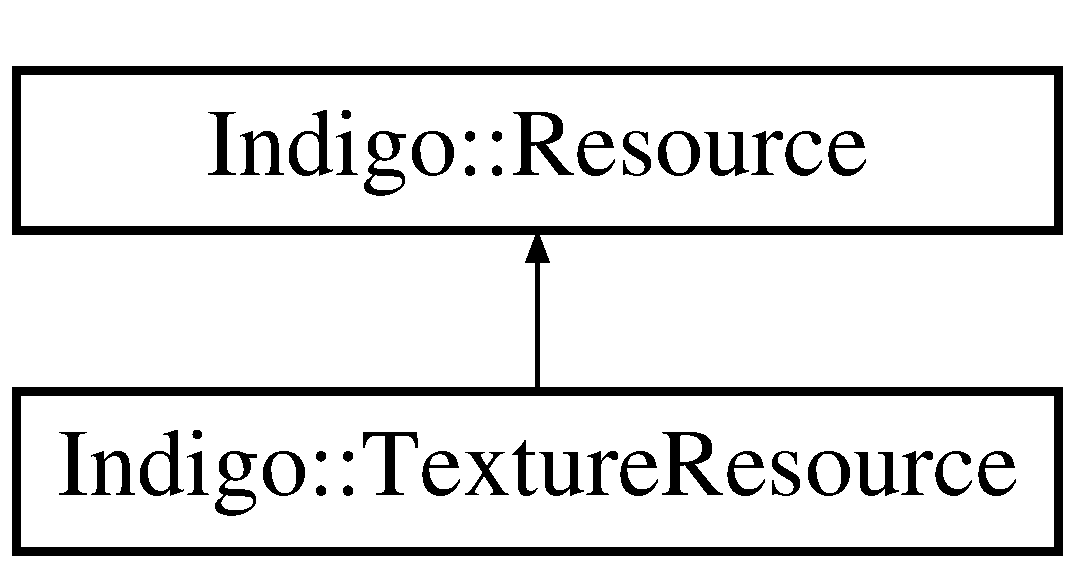
\includegraphics[height=2.000000cm]{class_indigo_1_1_texture_resource}
\end{center}
\end{figure}
\subsection*{Friends}
\begin{DoxyCompactItemize}
\item 
\mbox{\Hypertarget{class_indigo_1_1_texture_resource_a74b3f77e4a7285c624d30192f9643876}\label{class_indigo_1_1_texture_resource_a74b3f77e4a7285c624d30192f9643876}} 
class {\bfseries Resources}
\end{DoxyCompactItemize}


The documentation for this class was generated from the following file\+:\begin{DoxyCompactItemize}
\item 
src/indigo/Texture\+Resource.\+h\end{DoxyCompactItemize}

\hypertarget{class_indigo_1_1_transform}{}\section{Indigo\+:\+:Transform Class Reference}
\label{class_indigo_1_1_transform}\index{Indigo\+::\+Transform@{Indigo\+::\+Transform}}
Inheritance diagram for Indigo\+:\+:Transform\+:\begin{figure}[H]
\begin{center}
\leavevmode
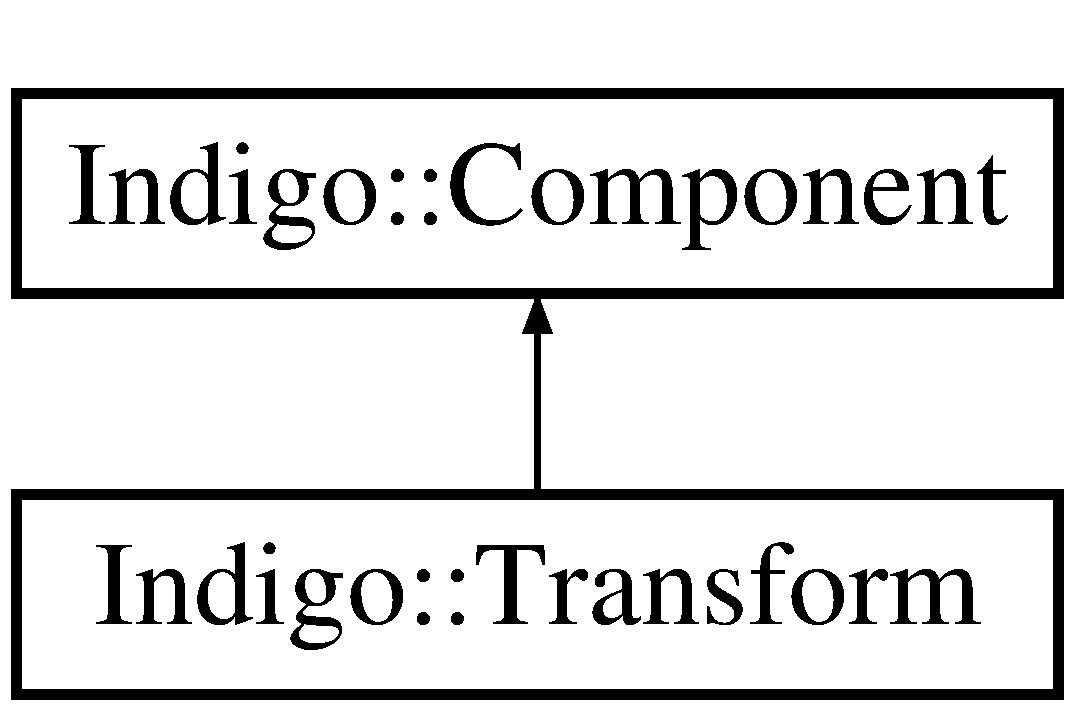
\includegraphics[height=2.000000cm]{class_indigo_1_1_transform}
\end{center}
\end{figure}
\subsection*{Public Member Functions}
\begin{DoxyCompactItemize}
\item 
\mbox{\Hypertarget{class_indigo_1_1_transform_ab1aaf133b18dcd920fcdcbe93edc548e}\label{class_indigo_1_1_transform_ab1aaf133b18dcd920fcdcbe93edc548e}} 
{\bfseries Transform} (glm\+::vec3 \+\_\+pos, glm\+::vec3 \+\_\+rot, glm\+::vec3 \+\_\+scale)
\item 
\mbox{\Hypertarget{class_indigo_1_1_transform_a71ade761a10a7ae77567928a36021320}\label{class_indigo_1_1_transform_a71ade761a10a7ae77567928a36021320}} 
glm\+::vec3 {\bfseries Get\+Position} ()
\item 
\mbox{\Hypertarget{class_indigo_1_1_transform_a0c9d4e095d96472142732b4f06219e8f}\label{class_indigo_1_1_transform_a0c9d4e095d96472142732b4f06219e8f}} 
glm\+::vec3 {\bfseries Get\+Rotation} ()
\item 
\mbox{\Hypertarget{class_indigo_1_1_transform_a42d36bf23efe1a84d28d54a6784f6eb0}\label{class_indigo_1_1_transform_a42d36bf23efe1a84d28d54a6784f6eb0}} 
glm\+::vec3 {\bfseries Get\+Scale} ()
\item 
\mbox{\Hypertarget{class_indigo_1_1_transform_aa4ffc305632fa25aeed22524b36e3e79}\label{class_indigo_1_1_transform_aa4ffc305632fa25aeed22524b36e3e79}} 
void {\bfseries Set\+Position} (glm\+::vec3 \+\_\+p)
\item 
\mbox{\Hypertarget{class_indigo_1_1_transform_a7e7618374106c5df66f8831d109c598f}\label{class_indigo_1_1_transform_a7e7618374106c5df66f8831d109c598f}} 
void {\bfseries Set\+Rotation} (glm\+::vec3 \+\_\+r)
\item 
\mbox{\Hypertarget{class_indigo_1_1_transform_a221016e4719c6e990bbe98e0e581f926}\label{class_indigo_1_1_transform_a221016e4719c6e990bbe98e0e581f926}} 
void {\bfseries Set\+Scale} (glm\+::vec3 \+\_\+s)
\item 
\mbox{\Hypertarget{class_indigo_1_1_transform_aefe0c69065a9870dc0c49d297dc316c5}\label{class_indigo_1_1_transform_aefe0c69065a9870dc0c49d297dc316c5}} 
glm\+::vec3 {\bfseries Get\+Forward} ()
\item 
\mbox{\Hypertarget{class_indigo_1_1_transform_a9d87de590be3b413b962ca5a1c90c0ef}\label{class_indigo_1_1_transform_a9d87de590be3b413b962ca5a1c90c0ef}} 
glm\+::vec3 {\bfseries Get\+Up} ()
\item 
\mbox{\Hypertarget{class_indigo_1_1_transform_a7e34c4791358814412983d8606cc4cdf}\label{class_indigo_1_1_transform_a7e34c4791358814412983d8606cc4cdf}} 
glm\+::vec3 {\bfseries Get\+Right} ()
\item 
\mbox{\Hypertarget{class_indigo_1_1_transform_ad4d433d8ecad0eb730be4294c57938db}\label{class_indigo_1_1_transform_ad4d433d8ecad0eb730be4294c57938db}} 
glm\+::mat4 {\bfseries Get\+Model\+Mat} ()
\item 
\mbox{\Hypertarget{class_indigo_1_1_transform_a2b3b2d50122bf966469832d5fc361834}\label{class_indigo_1_1_transform_a2b3b2d50122bf966469832d5fc361834}} 
void {\bfseries Translate} (glm\+::vec3 \+\_\+by)
\item 
\mbox{\Hypertarget{class_indigo_1_1_transform_a78633ea6630bd3ce493529ff122354e6}\label{class_indigo_1_1_transform_a78633ea6630bd3ce493529ff122354e6}} 
void {\bfseries Move\+To} (glm\+::vec3 \+\_\+target, float \+\_\+alpha)
\item 
\mbox{\Hypertarget{class_indigo_1_1_transform_a0d837c0a1d80c8e249e854c584b4b728}\label{class_indigo_1_1_transform_a0d837c0a1d80c8e249e854c584b4b728}} 
void {\bfseries Move\+Dir} (glm\+::vec3 \+\_\+dir, float \+\_\+alpha)
\item 
\mbox{\Hypertarget{class_indigo_1_1_transform_a41b24ff268187636f66dfa65432bda3a}\label{class_indigo_1_1_transform_a41b24ff268187636f66dfa65432bda3a}} 
void {\bfseries Rotate} (glm\+::vec3 \+\_\+euler\+Angles)
\item 
\mbox{\Hypertarget{class_indigo_1_1_transform_abb94f1c5b70ed256da1629130d680dee}\label{class_indigo_1_1_transform_abb94f1c5b70ed256da1629130d680dee}} 
void {\bfseries Scale} (glm\+::vec3 \+\_\+scale\+By)
\item 
\mbox{\Hypertarget{class_indigo_1_1_transform_a3256c0fb53d0b341ad8d80fe61e5fb2d}\label{class_indigo_1_1_transform_a3256c0fb53d0b341ad8d80fe61e5fb2d}} 
void {\bfseries Update} ()
\item 
\mbox{\Hypertarget{class_indigo_1_1_transform_ae62954b4df267cc4c7a1a837e1f9e5c0}\label{class_indigo_1_1_transform_ae62954b4df267cc4c7a1a837e1f9e5c0}} 
bool {\bfseries \+\_\+\+Check\+For\+A\+A\+B\+B\+Recalc} ()
\end{DoxyCompactItemize}
\subsection*{Friends}
\begin{DoxyCompactItemize}
\item 
\mbox{\Hypertarget{class_indigo_1_1_transform_a3e1914489e4bed4f9f23cdeab34a43dc}\label{class_indigo_1_1_transform_a3e1914489e4bed4f9f23cdeab34a43dc}} 
class {\bfseries Engine}
\end{DoxyCompactItemize}
\subsection*{Additional Inherited Members}


The documentation for this class was generated from the following files\+:\begin{DoxyCompactItemize}
\item 
src/indigo/Transform.\+h\item 
src/indigo/Transform.\+cpp\end{DoxyCompactItemize}

%--- End generated contents ---

% Index
\backmatter
\newpage
\phantomsection
\clearemptydoublepage
\addcontentsline{toc}{chapter}{Index}
\printindex

\end{document}
